% Part A: DC sweep of Vin. VTC. Explain observations.

\FloatBarrier

\begin{figure}[h!]
	\centering
	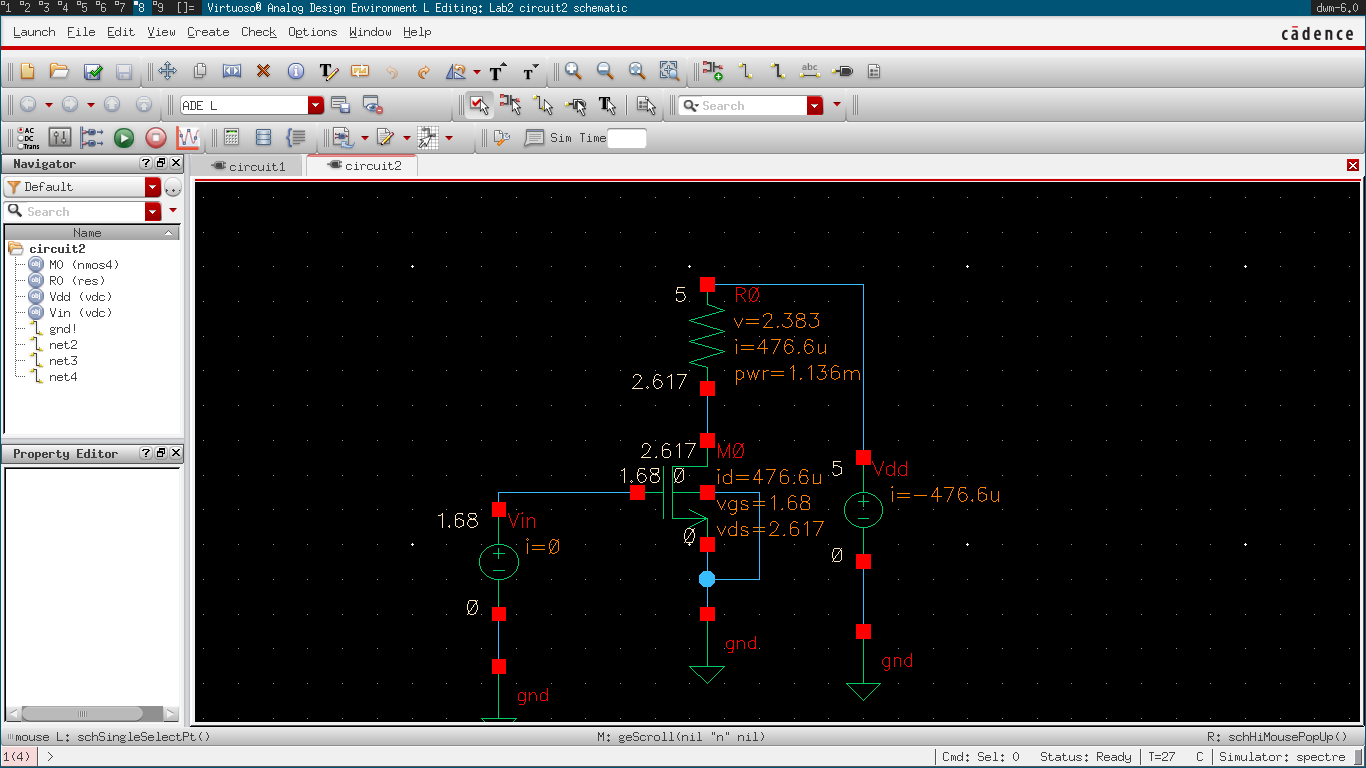
\includegraphics[scale=0.75]{../images/circuit2.PNG}
	\caption{Common-Source Amplifier}
	\label{fig:circuit2}
\end{figure}

\FloatBarrier

\FloatBarrier

\begin{figure}[h!]
	\centering
	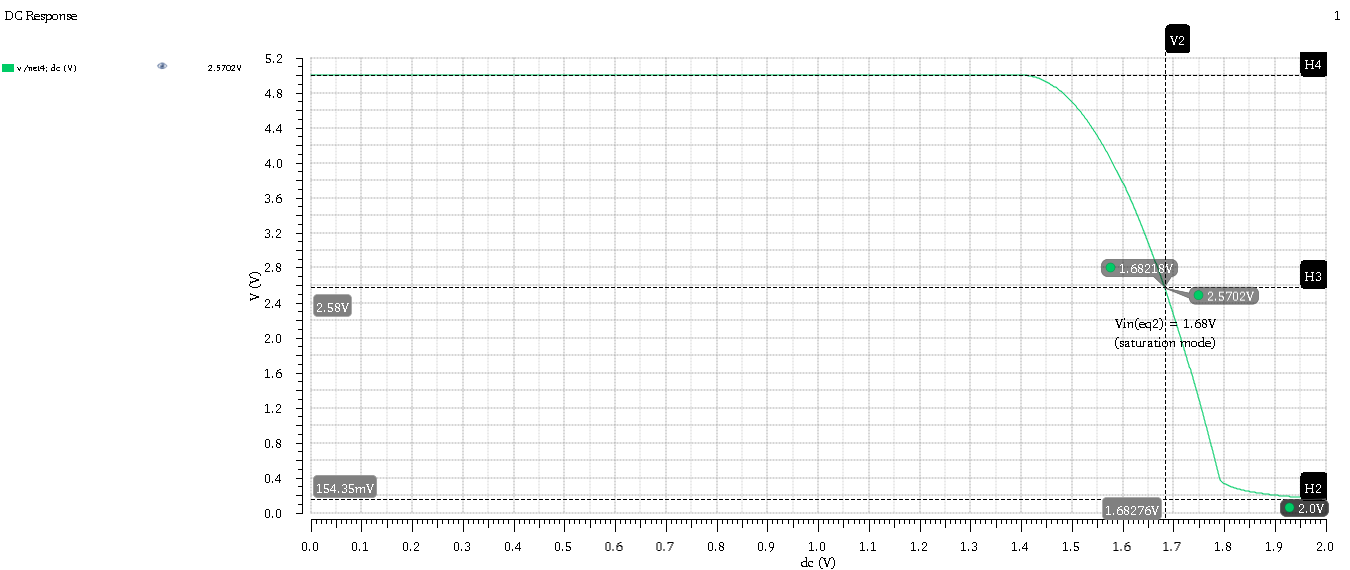
\includegraphics[scale=0.75]{../images/sim2_vtc.PNG}
	\caption{Voltage Transfer Characteristic for Common-Source Amplifier}
	\label{fig:sim2_vtc}
\end{figure}

\FloatBarrier
% Part B: Find V_in = V_ineq2
$V_{in(eq2)} = 1.68$\si{\volt} for this particular amplifier.
% In what region does the transistor operate?
The transistor operates in the saturation region at this point.
Common-source amplifiers start in cutoff mode for $V_{in}$ below the threshold voltage $V_{tn}$.
When $V_{in}$ is too large, they typically enter the triode mode.
For the region in between these two modes, the amplifier operates in saturation.
% DC op pt sim
Figure (\ref{fig:circuit2}) shows the results of a DC operating point simulation.
% Part C: Find gm and ro
These results can be used to calculate $g_{m}$.

\FloatBarrier

\begin{table}[h!]
	\centering
	\caption{$g_{m}$ for Common-Source Amplifier}
	\label{tab:common_source_amp_gm}
	\csvautotabular{../tables/common_source_amp_gm.csv}
\end{table}

\FloatBarrier
